\documentclass[Integrationstest/Integrationstest_main.tex]{subfiles}
\begin{document}

\lstdefinestyle{customc}{
    breaklines=true,
    language=C,
    showstringspaces=false,
}
\lstset{style=customc}

\section{WebPage og RPi integrationstest}
\subsection{Introduktion}
Modulet WebPage har til opgave at modtage brugerinputs i form af brugernavne, holdnavne og holdfarver og sende disse til GameController klassen. Herfra skal de videreformidles til resten af systemet, herunder playersides og display. Det er vigtigt at WebPage sender de rigtige informationer, og at der sjældent sker fejl i afsendingen. \\\\Det er ikke tilstrækkeligt kun at teste WebPage isoleret, da den baserer sig på kommunikation med GameController klassen og er afhængig af denne. WebPage er en boundary klasse til GameController, og det skal testes, at kommunikationen mellem klasserne forløber som planlagt. GameController klassen er imidlertid kompleks og varetager  mange af spillets funktioner. Der er derfor udviklet et separat program til formålet. Denne test stub skal simulere GameController klassen, så det kan undersøges, om GameController modtager de rigtige informationer, når de sendes fra hjemmesiden. 

\subsection{Integrationstest}
Der implementeres en C++ klasse kaldet WebPage og en C++ klasse kaldet GameController. Der anvendes den event drevne arkitektur, som er beskrevet i afsnittet "Design af RPiApp - USER SPACE". Det betyder at programmet anvender messages og message queues, samt klasserne Thread og ThreadFunctor til at håndtere tråde. I main oprettes GameControllers MsgQueue samt to tråde, hhv. WebPageThread og GameThread. Dette er vist i kodeeksemplet nedenfor.
\begin{lstlisting}
int main()
{
    MsgQueue GameControllerMsgQueue_;
    GameController GameControllerObj_(&GameControllerMsgQueue_);
    WebPage WebPageObj_(&GameControllerMsgQueue_);

    Thread GameThread(&GameControllerObj_);
    Thread WebPageThread(&WebPageObj_);

    GameThread.start();
    WebPageThread.start();
	
    GameThread.join();
    WebPageThread.join();
}
\end{lstlisting}
WebPageThread lytter på port 3000, og når der genereres et event fra client, dvs. der trykkes start på hjemmesiden sendes informationerne først til web serveren, som skal behandle data og konvertere det til det rigtige format. Hertil anvendes klassen UserInfo, som opbevarer hold- og brugernavne som strings og RGB værdier som 8 bit unsigned integers. Der oprettes nu en dynamisk allokeret besked kaldet WebPageRespone, som nedarver fra en Message klasse. Dette er i overensstemmelse med den event drevne arkitektur beskrevet i software design afsnittet "Design af RPiApp". WebPageResponse indeholder to objekter af klassen UserInfo, henholdsvis team1\_ og team2\_.  
Denne sendes til GameControllers beskedkø med det specifikke besked ID ID\_INFO\_READY, som er en del af MsgProtocol for RPiApp. Bemærk at WebPage har kendskab til beskedkøen, da den modtager en reference til denne, når den instantieres. I GameController tråden kører et special while loop, og når beskeden modtages sørger dispatcher systemet for at switche ud på beskedens ID. I dette tilfælde bliver informationerne for hold 1 og hold 2 udskrevet i terminalen, så det kan bekræftes, at kommunikationen forløber korrekt, og at data er som forventet. Dele af dispatcheren og handleren fremgår nedenfor. I handleren castes beskeden til en WebPageResponse *. På denne vis kan man tilgå get()-metoderne i UserInfo og udskrive værdierne for members for henholdsvis team1\_ og team2\_.
\begin{lstlisting}
void GameController::dispatcher(unsigned long messageID, Message * msg)
{
    switch (messageID) 
    {
        case ID_INFO_READY:
        {
	WebPageResponse * ind = static_cast<WebPageResponse *>(msg);

	std::cout << "Team 1:" << std::endl;
	std::cout << "Teamname is: " << ind->team1_.getTeam() << std::endl;
	std::cout << "Username1 is: " << ind->team1_.getUser1() << std::endl;
	std::cout << "Username2 is: " << ind->team1_.getUser2() << std::endl;
	std::cout << "Red is: " << ind->team1_.getRed() << std::endl;
	std::cout << "Green is: " << ind->team1_.getGreen() << std::endl;
	std::cout << "Blue is: " << ind->team1_.getBlue() << std::endl << std::endl;

	std::cout << "Team 2:" << std::endl;
	...
    	}
    }
}
\end{lstlisting}

\subsubsection{Fremgangsmetoden for test}
\begin{enumerate}
    \item Kompiler programmet på host
    \item Overfør den eksekverbare fil til RPi 
    \item Afvikl ekseverbar fil på target
    \item Log på netværk med SSID Beer\_Pong\_Table på smartphone
    \item Åbn hjemmesiden med ip-adresse 10.9.8.2
    \item Indtast holdoplysninger og tryk 'Start'
    \item Undersøg og dokumenter data sendt og modtaget 
\end{enumerate}

\subsubsection{Resultater}
Figur \ref{fig:Integration_1} viser hjemmesidens interface i browseren og resultatet af testen er vist med et terminal output i figur \ref{fig:Integration_2}. Det fremgår at holdnavne, brugernavne og holdfarver er sat som forventet.

\begin{figure}[H]
    \centering
    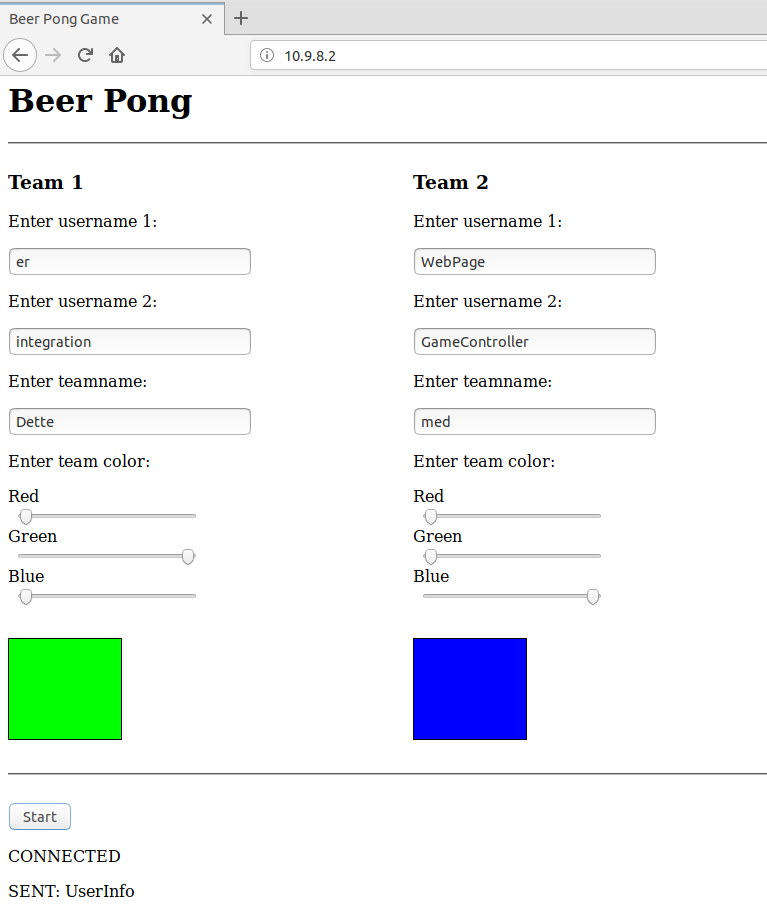
\includegraphics[width=0.9\textwidth]{Integrationstest/WebPageogRPi/graphics/integrationstest1_web_game.png}
    \caption{Integrationstest af WebPage og RPi - hjemmeside vist i browser}
    \label{fig:Integration_1}
\end{figure}
\begin{figure}[H]
    \centering
    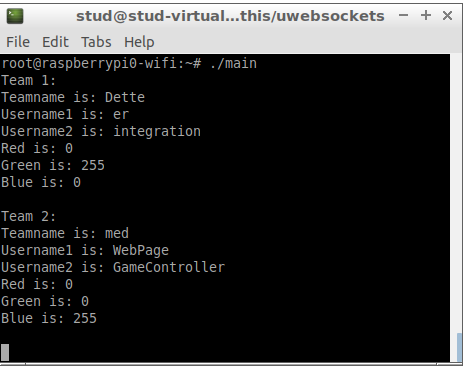
\includegraphics[width=\textwidth]{Integrationstest/WebPageogRPi/graphics/integrationstest2_web_game.png}
    \caption{Integrationstest af WebPage og RPi - output vist i terminal}
    \label{fig:Integration_2}
\end{figure}

\begin{figure}[H]
    \centering
    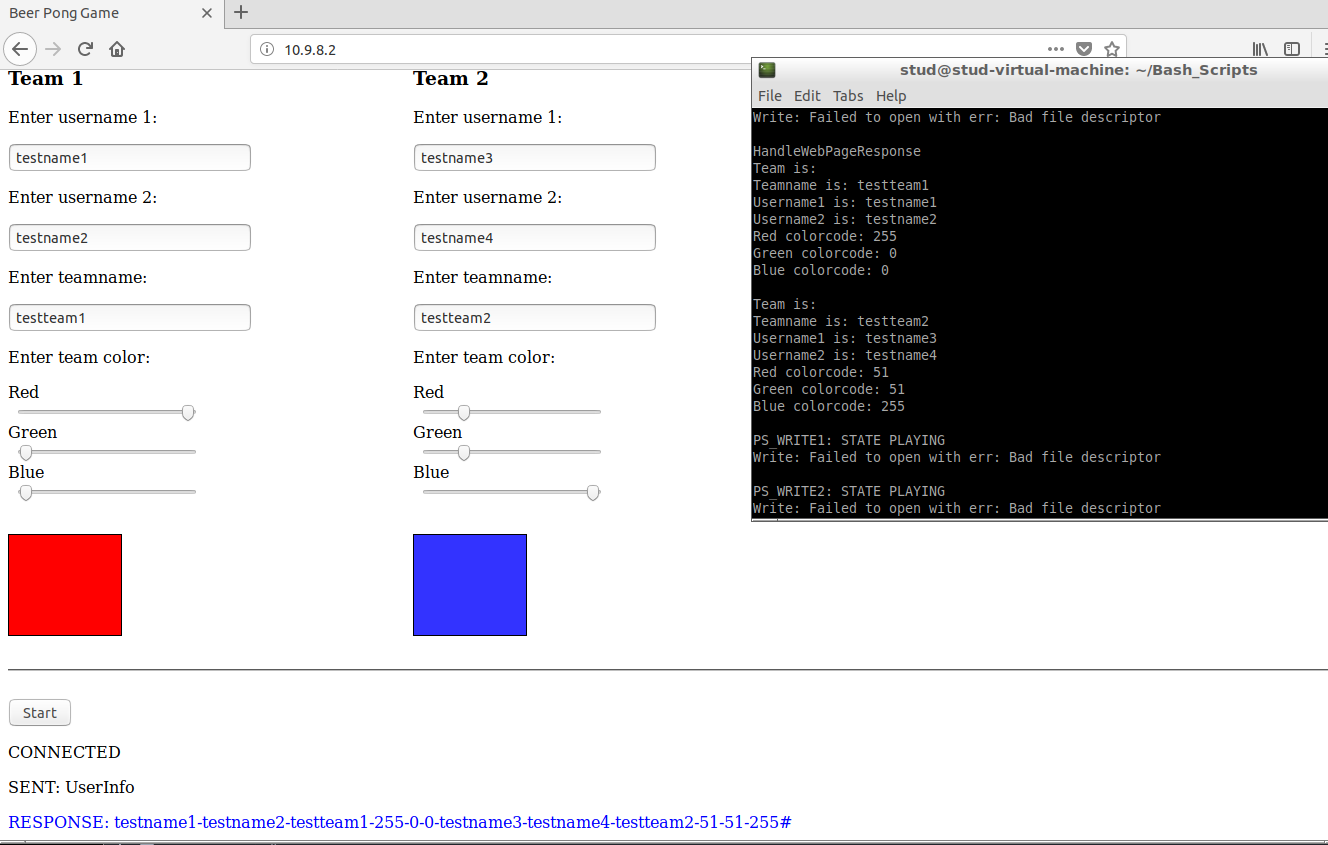
\includegraphics[width=1\textwidth]{Integrationstest/WebPageogRPi/graphics/webserver.png}
    \caption{Integrationstest af WebPage og RPi - output fra terminal og på WebPage GUI}
    \label{fig:Integration_3}
\end{figure}

\section{Reflektion}
Der opstod flere komplikationer under testen. De var dog alle af mindre karakter, og blev løst løbende. F.eks. var der uforudsete problemer med at konvertere rgb værdierne fra strings til uint8\_t og at udskrive disse i terminalen. De var imidlertid hurtigt løst og selve kommunikationen mellem WebPage og GameController viste sig at fungere som forventet. Som beskrevet i afsnittet 'Server' under Softwaredesign for boundary-klassen WebPage er kommunikationen bevidst gjort envejs. Dette designvalg kom os muligvis til gode under integrationstesten, da det har sænket kompleksiteten og elimineret visse fejlkilder. Når der trykkes 'Start' i client og data sendes, forbliver WebSocket forbindelsen åben. Der kunne således testes ved at sende gentagende beskeder, med varierende hold- og brugernavne samt farvevalg. Dette forløb efter hensigten og stemte overens med terminal outputs. 

\section{Konklusion}
Integrationstesten bekræftede, at GameController modtager de rigtige brugerinputs fra hjemmesiden, herunder hold- og brugernavne samt holdfarver. Den event drevne arkitektur lader til at være en hensigtsmæssig måde for de uafhængige tråde at kommunikere på. Klassen UserInfo indeholder informationerne, og måden hvorpå to objekter af denne bliver sendt ved hjælp af beskedsystemet virker også som forventet.
\end{document}